\section{Preliminaries}
\subsection{Notation}
The set of integers and real numbers are denoted $\int$ and $\real$ respectively. A ranged subset of a space is denoted with $\mathbb{S}\rii{i}{j}=\{s\in\mathbb{S}|i\leq s\leq j\}$. Parenthesis are used in place of brackets to denote strict inequalities. Open bounds are defined using notation such as $\mathbb{S}\rgeq{i}$ where any comparison operator can be substituted for $\geq$. A set of integers starting at 1 and going to $k\in\int\rgeq{1}$ is denoted with $\idxset{k}\triangleq\int\rii{1}{k}$. Use $\PowerSet{\cdot}$ to denote the power set of a set. 

Let $\mathcal{S}=\{\{\{\mathcal{S}_{(i,j,k)}\}_{k\in\mathcal{I}_{K}(i,j)}\}_{j\in\mathcal{I}_{J}(i)}\}_{i\in\mathcal{I}_I}$, $\mathcal{S}\subseteq\real^n$ be a nested collection of subsets of the $n$-dimensional, real-valued numbers. The first and second level sub-collections are denoted as $\mathcal{S}_{(i)}=\{\{\mathcal{S}_{(i,j,k)}\}_{k\in\mathcal{I}_{K}(i,j)}\}_{j\in\mathcal{I}_{J}(i)}$ and $\mathcal{S}_{(i,j)}=\{\mathcal{S}_{(i,j,k)}\}_{k\in\mathcal{I}_{K}(i,j)}$. Operations preformed between nested collections require the collections be of equal size and are preformed elementwise. For example, $\mathcal{S}_{(i)}$ equals $\tilde{\mathcal{S}}_{(i)}$ if they are the same size and every element in both is equivalent. Operations preformed between a nested collection and a single element behave as if the single element where an appropriate sized collection with elements equal to the single element. For example, setting $\mathcal{S}=\underline{0}$ sets every element of $\mathcal{S}$ to $\underline{0}$. Finally, union operations are preformed on every element of the nested collection. For example, $\cup \mathcal{S}_{(i)}$ is the union of all the elements of $\mathcal{S}_{(i)}$.

\subsection{Directed Graphs}
A directed graph, $\graph$, is comprised of $\gnumnodes\in\int\geq{1}$ nodes. Node $i\in\idxset{\gnumnodes}$ is defined by a list of edges leading to successor nodes, $\gnodeedges{i}\in\PowerSet{\idxset{\gnumnodes}}$, and a label, $\gnodelabel{i}=\idxset{\gnumlabels}^n$, where $\gnumlabels$ is the number of labels in the graph. If $j\in\mathcal{E}_i$, then transitioning from node $i$ to node $j$ is valid in a single time step. A time varying function mapping to nodes, $f:\int\rgeq{0}\rightarrow\idxset{\gnumnodes}$, is said to respect a graph $\mathcal{G}$ if $f(t)=i$ implies that $f(t+1)\in\gnodeedges{i}$. A time varying function mapping to labels, $g:\int\rgeq{0}\rightarrow\idxset{\gnumlabels}$, is said to respect a graph $\mathcal{G}$ if  there exists a function respecting $\mathcal{G}$, $f(t)$, such that $g(t)=\gnodelabel{f(t)}$. The set of all such functions is denoted $\Sigma(\mathcal{G})\triangleq\{g:\int\rgeq{0}\rightarrow\idxset{\gnumlabels}\ |\ g(\cdot)\text{ respects }\graph\}$. 

\subsection{Switching Signals}
An external switching signal is any function mapping the current time to some index, $\ss:\int\rgeq{0}\rightarrow\int\rii{1}{\nummodes}$. This work does not require prior knowledge of the switching signal but does assume its value at time $t$ is known immediately. Furthermore, the switching signal can be constrained to respect some known graph, $\ss\in\Sigma(\graph)$, where $\gnumlabels=\nummodes$. 
\begin{remark}
This is a generalizations of dwell time and successor constraints from previous literature that allows a richer set of constraints to be represented. For example, the graph below represents a 2-mode system where the first mode has a minimum dwell time of 2 while the second mode can only be left during odd dwell times.
\begin{figure}[h!]
\centering
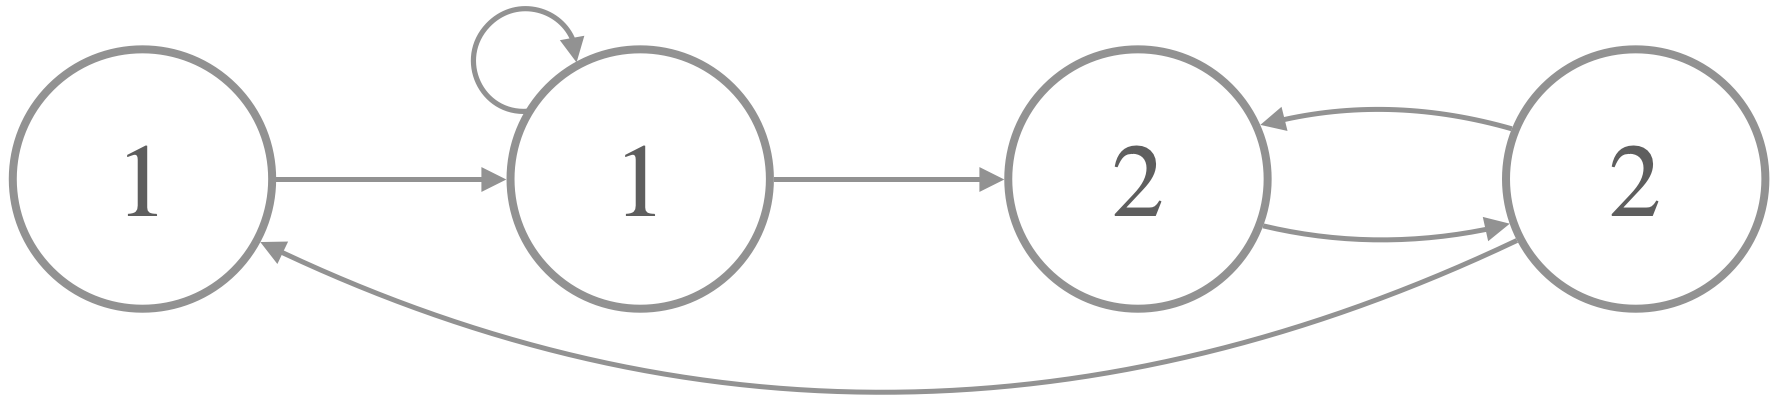
\includegraphics[scale=0.15]{./figures/graph_remark}
\end{figure}
\end{remark}

\subsection{Set Operations and Control Invariance}
Set operations provide tools to analyze how a system can evolve under allowable inputs. Given a linear system with additive disturbances and state and input constraints, $\mode{\modeidx}\triangleq\{A_\modeidx, B_\modeidx, E_\modeidx,\xcon[\modeidx],\ucon[\modeidx]\}$ where $x(t+1)=A_\modeidx x(t)+ B_\modeidx u(t)+ E_\modeidx w(t)$, the following important set operations are introduced. 
\begin{definition}[Robust Preset]\label{def:robust_preset}
The $k$-step, robust preset of a set $\mathcal{S}$ under the constrained dynamics $\mode{\modeidx}$ and disturbance constraint $w\in\wcon$ is given by
\begin{align}
\Pre[\modeidx][0]{\mathcal{S},\wcon}&\triangleq\mathcal{S},\\
\Pre[\modeidx][k]{\mathcal{S},\wcon}&\triangleq\{x\in\xcon\ |\ \exists u\in\ucon\text{ s.t. }\forall w\in\wcon,\nonumber\\ &A_\modeidx x+ B_\modeidx u+ E_\modeidx w\in\Pre[\modeidx][k-1]{\mathcal{S},\wcon}\}.
\end{align}
\end{definition}
\begin{definition}[Previewed Robust Preset]\label{def:prev_robust_preset}
The $k$-step, previewed robust preset of a set $\mathcal{S}$ under the constrained dynamics $\mode{\modeidx}$ and disturbance constraint $w\in\wcon$ is given by
\begin{align}
\PreviewedPre[\modeidx][0]{\mathcal{S},\wcon}&\triangleq\mathcal{S},\\
\PreviewedPre[\modeidx][k]{\mathcal{S},\wcon}&\triangleq\{x\in\mathcal{X}|\forall w\in\mathcal{W},\exists u\in\mathcal{U}\text{ s.t. }\nonumber\\
&A_\modeidx x+ B_\modeidx u+ E_\modeidx w\in\PreviewedPre[\modeidx][k-1]{\mathcal{S},\wcon}\}.
\end{align}
\end{definition}
The previewed robust presets are used when the system is allowed a preview of the current disturbance. This preview can expand the size of the preset because the selected input need not handle every possible disturbance. Robust presets both with and without previews can be found using basic set operation such as the Minkowski sum and difference as shown below \cite{Borrelli2017}.
\begin{align}
\Pre[][1]{\mathcal{S}} &= \left(\left(\left(\mathcal{S}\ominus A_w\circ\mathcal{W}\right)\oplus\left(-B\circ\mathcal{U}\right)\right)\circ A\right)\ \cap\ \mathcal{X},\\
\PreviewedPre[][1]{\mathcal{S}} &= \left(\left(\left(\mathcal{S}\oplus\left(-B\circ\mathcal{U}\right)\right)\ominus A_w\circ\mathcal{W}\right)\circ A\right)\ \cap\ \mathcal{X}.
\end{align}

Preset operations are critical in the calculation of invariant sets commonly used in feasibility analysis. An invariant set is defined as follows.
\begin{definition}[\Ac{ci} Set]\label{def:ci_set}
\alert{Add def}
\end{definition}

A final tool used in this paper is the convex hull of a set defined as follows.
\begin{definition}[Convex Hull]
\alert{add def}
\end{definition}
\subsection{Feasibility Analysis}
In constrained systems, it is extremely important that the controller can satisfy the state constraints using only feasibly inputs. If a feasible input exists such that the resulting state is also feasible, the system is feasible. If feasibility at the current time implies feasibility at all future times, then the system is persistently feasible.

In centralized unswitched systems, persistent feasibility can be established by constraining the system to be within a \ac{ci} set, $\mathcal{C}\subseteq\mathcal{X}$ \alert{cite}. Relying on constant, control invariant sets become difficult in externally switched systems, however. The \ac{ci} set must be common to all system modes else persistent feasibility is lost. This concern can be addressed using time varying, control invariant sets that take advantage of constraints on the switching signal. For example, in \cite{Danielson2019,Santis2004}, time varying, control invariant sets were developed that force the system to move during the dwell time between switches to a region from which a switch to any successor mode will preserve persistent feasibility. By lower bounding the dwell time, the system had additional time to reach these safe regions thereby loosening the state constraints. These results have been further expanded to include the robust case \cite{Lavaei2021}.

The ideas presented in the previous literature can be described using safe-set collections. These are collections of sets, indexed by some time varying signal, that serve as the active state constraints of the system. To establish persistent feasibility, every safe-set must be within the 1-step preset of all possible successor safe-sets. This is presented formally in the following definition.
\begin{definition}[Safe-set collection]
Let the external switching signal, $\ss\in\Sigma(\graph)$ govern the system $\mode{}(t)=\{f_{\ss(t)}(x(t),u(t)),\xcon[\ss(t)],\ucon[\ss(t)]\}$. A collection of sets indexed by the nodes of $\graph$, $\mathcal{S}=\{\mathcal{S}_{i}\}_{i\in\idxset{\gnumnodes}}$ is a safe-set collection if
$$\mathcal{S}_{i}\subseteq\Pre[\gnodelabel{j}][1]{\mathcal{S}_{j}}\ \forall\ i\in\idxset{\gnumnodes},\ j\in \gnodeedges{i}$$
\end{definition}
Safe set collections create target sets for the system to move into at each time step. The preset condition ensures that, no matter how $\ss$ evolves, the system will always be able to find a feasible input to move into the current target set.
